\label{chapter:chap3}

\begin{miniabstract}
Now, we will survey the maximum entropy multi-agent reinforcement learning (MEMARL) framework, which requires us to examine more deeply into each algorithms in control as probabilistic inference framework (MAPI). By re-derive the one of the algorithms ROMMEO \cite{tian2019regularized}, we understand how current MAPI operates, and what is the meaning of optimality. The main aim is to gain more understanding for the algorithms that will be used as a basis to construct others algorithms in this thesis.
\end{miniabstract}


\section{Introduction to MAPI framework}
\label{sec:chap3-intro-MAPI}

\subsection{What is MAPI ?}
All of the algorithms in MAPI frameworks are decentralized MARL algorithms. They are based on an opponent model but not a kind of opponent model in fictitious play \cite{berger2007brown}, where the agent assumes its opponent to be stationary as it tries to predict the opponent's move and best response to that opponent model. MAPI agents, instead, train its opponent model given its opponent reward. Since we know the agent's opponent model, we can reduce the multi-agent problem into a single-agent problem. During the training phase, we will assume that the action given by the real opponent comes from our assumed opponent model, and we train our agent accordingly. The difference between ROMMEO \cite{tian2019regularized} and PR2 \cite{wen2019probabilistic} happens when we define which component we optimize first. In ROMMEO's case, we train the agent's policy first then train the opponent model, and PR2 vice versa. Thus, we can view PR2's opponent model $\pi(a^{-i} | s, a^i)$ as an opponent's policy doing ROMMEO like training on its opponent (the agent) model $\pi(a^i | s)$. 

A training algorithm that incorporates the learning of the opponent model with the learning of the agent's policy can be beneficial in a cooperative case since both agent's policy and the real opponent (not agent's opponent model) try to optimize the same objective. However, this is also a weakness because if we have an opponent with drastically difference goal (for example in the case of a competitive game), the agent would still update its opponent model to act as if it is maximizing the agent's reward. The problem will be more apparent once we have understood the result on the impact of $\beta$s in theorem \ref{thm:update-balance-opponent}. We propose a solution that decouples the agent's training from the opponent's model. We have created an experiment showing how PR2 and ROMMEO fail to understand its opponent's action. We shall start with the payoff function, which is 
\begin{equation}
\label{eqn:chap3-matrix-game}
    R = \begin{bmatrix}
    2 & 3 & 3 \\
    1 & 4 & 0 \\
    1 & 0 & 10
    \end{bmatrix}
\end{equation}
If agent $i$ selects $a$ as its action and if agent $j$ selects $b$ as its action, then the reward of agent $i$, $r^i$, is $R_{ab}$ while the reward for agent $j$, $r^{j}$ is $-R_{ab}$. The Nash equilibrium is when agent $i$ selects action $1$ and agent $j$ selects action $1$ as their action, represented as $(1, 1)$, which would gives agent $i$ reward $2$ and $-2$ for agent $j$. Furthermore, in the cooperative case, where $r^{j} = R_{ab}$ there are 2 Nash equilibriums, which are $(2, 2)$ and $(3, 3)$, where Nash equilibrium at $(3, 3)$ is better. This game is similar to a climbing game proposed in \cite{claus1998dynamics} that is used in \cite{tian2019regularized}. While having similar property to the climbing game, the game we proposed has a pure Nash equilibrium at it zero-sum counter part. 

Let's start with training ROMMEO \cite{tian2019regularized} and PR2 \cite{wen2019probabilistic} on the cooperative setting. We calculate the action-value function $Q(a^j_t, a^{j}_t)$ using the stochastic update rule as following a stochastic updating rule presented in theorem \ref{thm:updaate-stochastic}. We also employ a temperature scheduling because during training due to reward differences the agent's policy converges prematurely. The details of the experiment will be discussed in appendix \ref{appx:chap4-matrix-game-explain}. The experiment results are collected by average over five experiments, each with different seeds. The baseline results are presented in figure \ref{fig:chap3_ROMMEO_PR2}. 
\begin{figure}
    \centering
    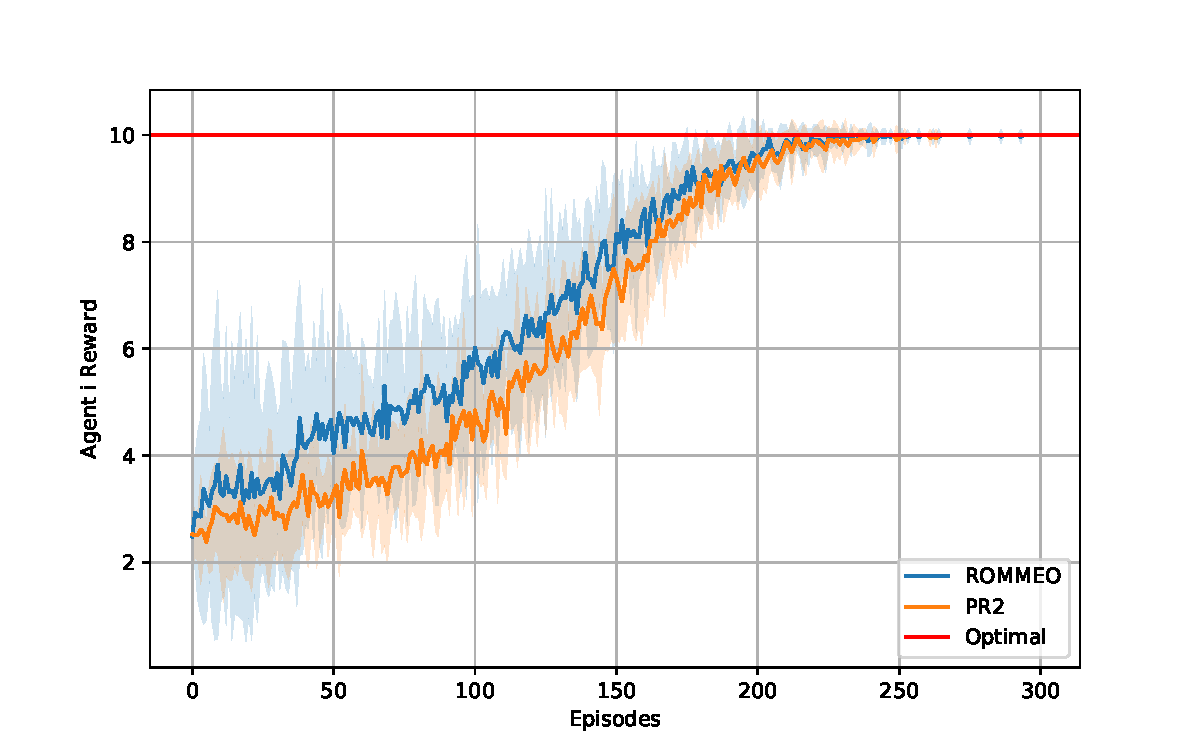
\includegraphics[scale=0.55]{figures/ROMMEO_PR2_ICG.pdf}
    \caption{The training progress of ROMMEO and PR2 on the cooperative game where the payoff is defined in equation \ref{eqn:chap3-matrix-game}.}
    \label{fig:chap3_ROMMEO_PR2}
\end{figure}
The reward of agent $j$ would be the same. We can see that ROMMEO does slightly better than PR2 as expected from the results presented in \cite{tian2019regularized}. We can see that due to the temperature schedule, the variances of both curves for the first 150 episodes are high, which is also a sign of exploration. Now, let's consider agent $i$ training when dealing with adversarial agent $j$ to study the impact of the variable $\beta^i$ and $\beta^j$ of agent $i$. We will follow the Balancing Q-learning algorithm, in which we have the following results shown in figure \ref{fig:chap3-comparison-balance-pr2-matrix}. First, in figure \ref{fig:chap3-balancing-q-min-max-matrix}, both agents converge to a Nash equilibrium when using Balancing Q-learning, which isn't the case for PR2. By misrepresentation of its opponent, agent $i$ trained under PR2 algorithm will choose action $3$ (since in cooperative case this is the best action) giving a lower reward of almost $0$ leading to suboptimal performance. On the other hand, agent $i$ that is trained under Balancing-Q will choose action $1$ yielding the reward of $2$, and reaches Nash equilibrium. 
\begin{figure}[h]
\centering
\begin{subfigure}{.5\textwidth}
  \centering
  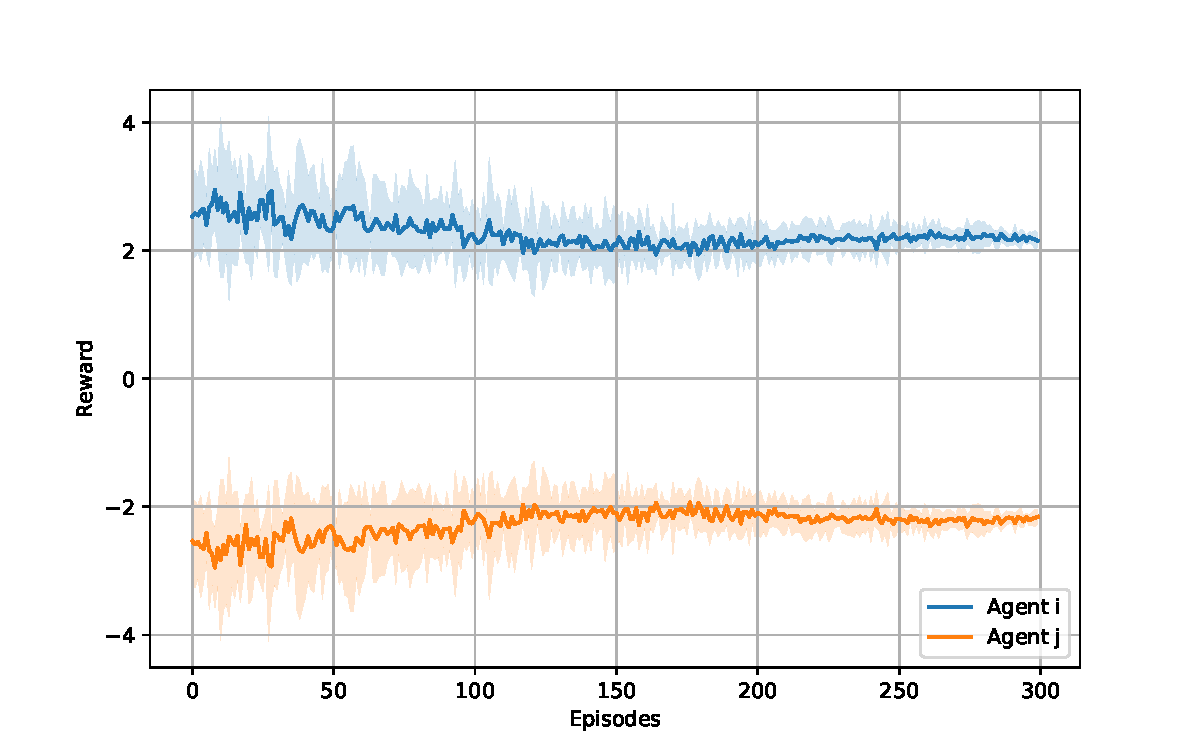
\includegraphics[width=\linewidth]{figures/Balancing_correct.pdf}
  \caption{Balancing Q-learning with adversarial opponent}
  \label{fig:chap3-balancing-q-min-max-matrix}
\end{subfigure}%
\begin{subfigure}{.5\textwidth}
  \centering
  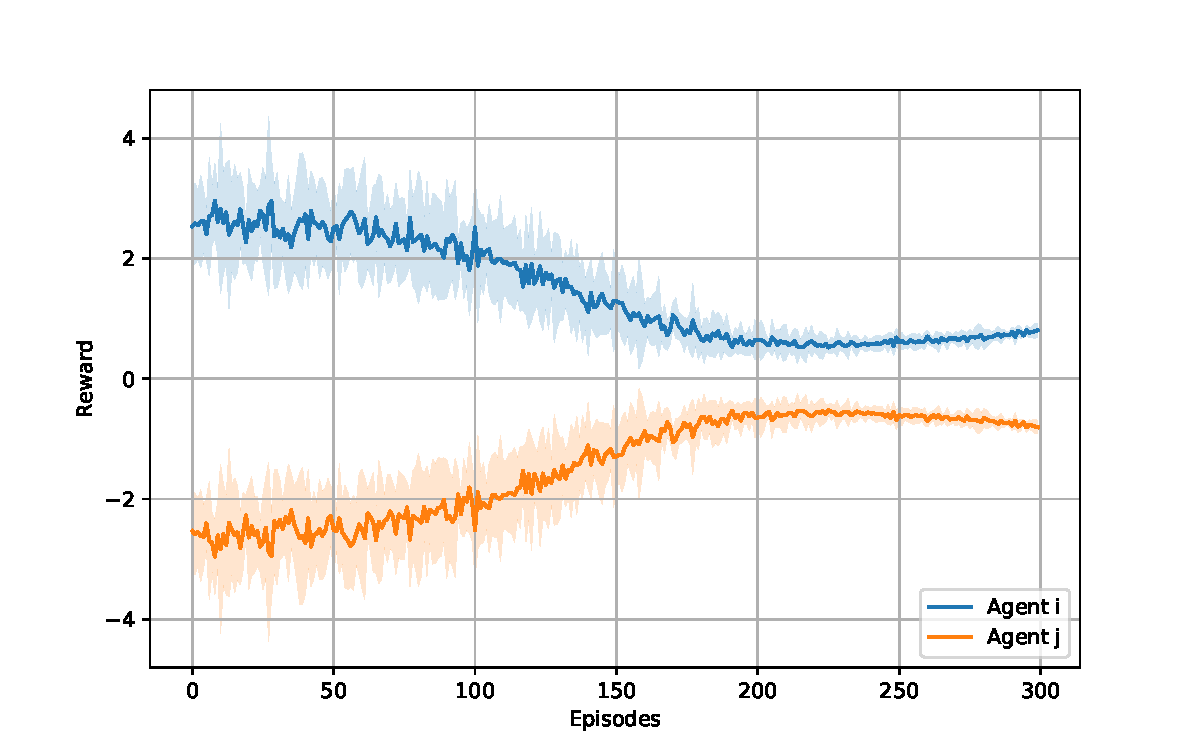
\includegraphics[width=\linewidth]{figures/Balancing_wrong.pdf}
  \caption{PR2 with misrepresentation of the opponent}
  \label{fig:chap3-pr2-min-max-matrix}
\end{subfigure}
\caption{A comparison between PR2 and Balancing Q-learning with adversarial opponent. PR2 can only represent cooperative opponent. Given the same set of seed the final reward are differ.}
\label{fig:chap3-comparison-balance-pr2-matrix}
\end{figure}

% Furthermore, one of the tricks that can be deployed to make the opponent model similar to the real opponent is to use supervised training on the prior opponent model given state and opponent action as a training set. By having a supervised opponent model, we can use it as a prior in our opponent model optimization as deployed in \cite{tian2019regularized}.

\subsection{What is Optimal ?}
We usually assume the optimality of the agent \textit{relative} to our knowledge of the opponent. If we are best responding to an optimal agent then we are likely to be optimal too\footnote{This is true in Nash equilibrium case by the definition.}. By jointly optimizing the agent with its opponent model, we can participate in what our opponent \textit{could be} given our assumptions and objective. This assumption is crucial, which will allow us to extend the framework so that it covers MAKL framework. We want to note that the assumption of an opponent's optimality is used in \cite{tian2019regularized}. However, it lacks the insight that the opponent's model doesn't have to follow the same objective as the agent, which we can show in the derivation of ROMMEO. In conclusion, MAPI is an enhanced probabilistic version of the fictitious play, where the opponent model is a fully trained policy. At the same time, the optimality of each agent should be independent while being based on each other, which is an inevitable contradiction but we will show that this is possible given special circumstances of Balancing Q-learning. 




\section{Derivation of ROMMEO}
Now, we shall consider the derivation of ROMMEO using the technique introduced in \cite{levine2018reinforcement}, which is shown briefly in section \ref{sec:chap2-derivation-soft-closed-form}. The working is partially covered in \cite{yu2019multi, wen2019multi} however a full derivation is required for the understanding of the algorithm. We will base our derivation for ROMMEO \cite{tian2019regularized}, while the same technique can be applied to PR2 \cite{wen2019probabilistic}. ROMMEO assumes that the joint probability between 2 agents, which can be factorized as
\begin{equation}
    \pi(a, a^{-i} | s) = \pi(a | a^{-i}, s) \rho(a^{-i} | s)
\end{equation}
factorizing in other ways yields PR2. We will start by drawing the graphical model of joint probabilities that we want to approximate, and is depicted in Figure \ref{fig:chap3-approximated-ROMMEO}. 
\begin{figure}[ht]
    \begin{minipage}[t]{0.5\linewidth}
    \centering
    \begin{tikzpicture}[latent/.append style={minimum size=1.5cm}]
        \node[obs] (ot) {$\mathcal{O}^i_t, \mathcal{O}^{-i}_t$};
        \node[latent, below=of ot] (at) {$a^{-i}_t$};
        \node[latent, below=of at] (st) {$s_t$};
        \node[latent, below=of st] (a1t) {$a^i_t$};
        % \node[obs, below=of a1t] (o1t) {$\mathcal{O}^i_t$};
        
        
        % \path[->]  (o1)  edge   [bend left=45] node {} (a);
        % \edge{o1t} {a1t}
        \edge {st} {at, a1t}
        \edge {at} {ot}
        % \path[->]  (o1t)  edge   [bend left=60] node {} (ot);
        \path[->]  (a1t)  edge   [bend left=45] node {} (ot);
        \path[->]  (a1t)  edge   [bend left=30] node {} (at);
        \path[->]  (st)  edge   [bend left=30] node {} (ot);
        
        \node[obs, right=3cm of ot] (ot1) {$\mathcal{O}^i_{t+1}, \mathcal{O}^{-i}_{t+1}$};
        \node[latent, below=of ot1] (at1) {$a^{-i}_{t+1}$};
        \node[latent, below=of at1] (st1) {$s_{t+1}$};
        \node[latent, below=of st1] (a1t1) {$a^i_{t+1}$};
        % \node[obs, below=of a1t1] (o1t1) {$\mathcal{O}^i_{t+1}$};
        
        % \edge{o1t1} {a1t1}
        \edge {st1} {at1, a1t1}
        \edge {at1} {ot1}
        % \path[->]  (o1t1)  edge   [bend right=60] node {} (ot1);
        \path[->]  (a1t1)  edge   [bend right=45] node {} (ot1);
        \path[->]  (a1t1)  edge   [bend right=30] node {} (at1);
        \path[->]  (st1)  edge   [bend right=30] node {} (ot1);
        
        \path[->]  (st)  edge   [] node {} (st1);
        \path[->]  (at)  edge   [] node {} (st1);
        \path[->]  (a1t)  edge   [] node {} (st1);
        
        \node[latent, right=5cm of st1] (stn) {$s_{t+n}$};
        \path[->]  (st1)  edge [] node {} (stn);
    \end{tikzpicture}
    \end{minipage}%
    \begin{minipage}[t]{0.5\linewidth}
    \caption{Graphical model that we want to approximate. This is based on the joint probability provided in ROMMEO paper, with slight modification. The authors assume that the opponent we are playing against is optimal}
    \label{fig:chap3-approximated-ROMMEO}
    \end{minipage}
\end{figure}
Before we move on, please note that this is all within an agent calculation, while the opponent's policy will have the same process. Given this, we can show that the prior joint probability is equal to the following:
\begin{equation}
    \begin{aligned}
        P(s_{1:T}, &a^i_{1:T}, a^{-i}_{1:T}, \optim^{-i}_{1:T} = 1, \optim^{i}_{1:T} = 1) \\
        &= P(s_0) \prod^T_{t=0} P_{\prior}(a^i_t | s_t, a^{-i}_t) P_{\prior}(a^{-i}_t | s_t) P(s_{t+1} | s_t, a^i_t, a^{-i}_t) P(\optim^{-i}_t = 1, \optim^{i}_t = 1 | s_t, a^i_t, a^{-i}_t)
    \end{aligned}
\end{equation}
where the optimality variable is defined as 
\begin{equation}
\begin{aligned}
    &P(\optim_t^{-i} = 1, \optim^{i}_t = 1 | s_t, a^i_t, a^{-i}_t) \propto \exp \bracka{ \beta r(s_t, a^i_t, a^{-i}_t)  } \\
    &P(\optim_t^{-i} = 1, \optim^{i}_t = 1 | s_t, a^i_t, a^{-i}_t) = P(\optim_t^{-i} = 1 |\optim^{i}_t = 1, s_t, a^i_t, a^{-i}_t) P(\optim^{i}_t = 1 | \optim^{-i}_t = 1, s_t, a^i_t, a^{-i}_t)
\end{aligned}
\end{equation}
This definition is different from the one proposed in \cite{tian2019regularized}. However, we would like to point out that the opponent model has been optimized \textit{after} the agent's policy, which will show in a later section. Therefore, during the optimization of the opponent model, it has assumed that the agent's policy is optimal, hence the factorization of the optimality. Furthermore, the factorization of the optimality random variables above is a mere representation because the distinction between agent's and its opponent model lies during the calculation of the solution and not during the inference. Now for the variational joint probabilities that we want to optimize on the graphical model is depicted in Figure \ref{fig:chap3-variational-ROMMEO}.
\begin{figure}[ht]
    \begin{minipage}[t]{0.5\linewidth}
    \centering
    \begin{tikzpicture}[latent/.append style={minimum size=1.0cm}]
        \node[latent] (at) {$a^i_t$};
        \node[latent, below=of at] (st) {$s_t$};
        \node[latent, below=of st] (a1t) {$a^{-i}_t$};
        
        % \edge{o1t} {a1t}
        \edge {st} {at, a1t}
        % \edge {at} {ot}
        % \path[->]  (o1t)  edge   [bend left=60] node {} (ot);
        % \path[->]  (a1t)  edge   [bend left=45] node {} (ot);
        \path[->]  (a1t)  edge   [bend left=30] node {} (at);
        % \path[->]  (st)  edge   [bend left=30] node {} (ot);
        
        % \node[obs, right=3cm of ot] (ot1) {$\mathcal{O}^i_{t+1}$};
        \node[latent, right=3cm of at] (at1) {$a^i_{t+1}$};
        \node[latent, below=of at1] (st1) {$s_{t+1}$};
        \node[latent, below=of st1] (a1t1) {$a^{-i}_{t+1}$};
        % \node[obs, below=of a1t1] (o1t1) {$\mathcal{O}^{-i}_{t+1}$};
        
        % \edge{o1t1} {a1t1}
        \edge {st1} {at1, a1t1}
        % \edge {at1} {ot1}
        % \path[->]  (o1t1)  edge   [bend right=60] node {} (ot1);
        % \path[->]  (a1t1)  edge   [bend right=45] node {} (ot1);
        \path[->]  (a1t1)  edge   [bend right=30] node {} (at1);
        % \path[->]  (st1)  edge   [bend right=30] node {} (ot1);
        
        \path[->]  (st)  edge   [] node {} (st1);
        \path[->]  (at)  edge   [] node {} (st1);
        \path[->]  (a1t)  edge   [] node {} (st1);
        
        \node[latent, right=5cm of st1] (stn) {$s_{t+n}$};
        \path[->]  (st1)  edge [] node {} (stn);
    \end{tikzpicture}
    \end{minipage}%
    \begin{minipage}[t]{0.5\linewidth}
    \caption{Graphical model that we are going to optimize our policies on. This has almost the same structure as the version that we want to approximate. However, we don't care about the optimality of the agent itself, as we want to approximate its policy (denote as $\pi$) and the its opponent model (denote as $\rho$)}
    \label{fig:chap3-variational-ROMMEO}
    \end{minipage}
\end{figure}
The joint probability of variational distribution can be calculated as following 
\begin{equation}
    q(s_{1:T}, a_{1:T}^i, a^{-i}_{1:T}) = P(s_0) \prod^T_{t=0} \pi_{\theta}(a^i_t | s_t, a^{-i}_t) \rho_{\phi}(a^{-i}_t | s_t) P(s_{t+1} | s_t, a^i_t, a^{-i}_t)P(\optim^{-i}_t = 1)
\end{equation}
We would like to solve the following optimization problem 
\begin{equation}
    \argmin{\pi, \phi \in \Pi \times \Phi}  \kl\bracka{q(s_{1:T}, a_{1:T}^i, a^{-i}_{1:T}) \Big\| P(s_{1:T}, a^i_{1:T}, a^{-i}_{1:T}|\optim^i_{1:T} = 1  \optim^{-i}_{1:T} = 1) }
\end{equation}
This leads to optimizing the following ELBO. The derivation is shown in the appendix \ref{appx:chap3-ROMMEO-ELBO}, which translates the problem into a maximization problem of the following objective
\begin{equation}
\label{eqn:chap3-ROMMEO-ELBO}
    \argmax{\pi, \phi \in \Pi \times \Phi} \mathbb{E}_{q}\brackb{ \sum^T_{t=0} \gamma^t\bracka{\beta r(s_t, a^i_t, a^{-i}_t)  - \log \frac{\pi_{\theta}(a^i_t | s_t, a^{-i}_t)}{P_{\prior}(a^i_t | s_t, a^{-i}_t) } - \log \frac{\rho_{\phi}(a^{-i}_t | s_t)}{P_{\prior}(a^{-i}_t | s_t)}}}
\end{equation}
We will start off by considering the last time step, as we will progress backwards in time. Considering the last time step:
\begin{equation}
\label{eqn:training-obj-last-time}
    \mathbb{E}_{q} \brackb{ \beta r(s_T, a^i_T, a^{-i}_T)  - \log \frac{\pi_{\theta}(a^i_T | s_T, a^{-i}_T)}{P_{\prior}(a^i_T | s_T, a^{-i}_T) } - \log \frac{\rho_{\phi}(a^{-i}_T | s_T)}{P_{\prior}(a^{-i}_T | s_T)}}
\end{equation}
We can show that the optimal policy is equal to 
\begin{equation}
\begin{aligned}
    &\pi_{\theta}(a^i_T | s_T, a^{-i}_T) = \frac{\exp \bracka{\beta r(s_t, a^i_T, a^{-i}_T)}P_{\prior}(a^i_T | s_T, a^{-i}_T)}{\exp\bracka{Q(s_T, a^{-i}_T)}} \\
    \text{where }& Q(s_T, a^{-i}_T) = \log \int \exp \bracka{\beta R(s_T, a^i_T, a^{-i}_T}P_{\prior}(a^i_T | s_T, a^{-i}_T)  \dby a^i_T
\end{aligned}
\end{equation}
The proof will be presented in the appendix \ref{appx:chap3-ROMMEO-agent-last-time}. This part is where we can assume that the agent policy is optimal and allow us to calculate the opponent model objective. By plugging the optimal policy back, we are left with the opponent's objective:
\begin{equation}
    \mathbb{E}_{ \rho_{\phi}(a^{-i}_T | s_T) P(s_T)}\brackb{ Q(s_T, a^{-i}_T) - \log \frac{\rho_{\phi}(a^{-i}_T | s_T)}{P_{\prior}(a^{-i}_T | s_T)} }
\end{equation}
which will give us the optimal opponent model at time step $T$ to be as the following:
\begin{equation}
\begin{aligned}
    &\rho_{\phi}(a^{-i}_T | s_T)  = \frac{ \exp\bracka{Q(s_T, a^{-i}_T)}P_{\prior}(a^{-i}_T | s_T) }{\exp\bracka{V(s_T)}}  \\
    \text{where }& V(s_T) = \log \int \exp\bracka{Q(s_T, a^{-i}_T)}P_{\prior}(a^{-i}_T | s_T) \dby a^{-i}_T
\end{aligned}
\end{equation}
All the proofs including the opponent's objective is in appendix \ref{appx:chap3-ROMMEO-opponent-last-time}. Given both agent and its opponent's model policy, we can consider the message passed to the time steps before, and we can see that we are left with
\begin{equation}
    \mathbb{E}_{P(s_T)}\brackb{V(s_T)}
\end{equation}
This quantity will be passed down to the later time. Now for time $t$, the objective that we are optimizing becomes 
\begin{equation}
    \mathbb{E}_{q} \Bigg[ \underbrace{\beta r(s_t, a^i_T, a^{-i}_T) + \gamma \mathbb{E}_{P(s_{t+1} | s_t, a^i_t, a^{-i}_t)}  \brackb{V(s_{t+1})}}_{Q(s_t, a^i_t, a^{-i}_t)}  - \log \frac{\pi_{\theta}(a^i_T | s_t, a^{-i}_t)}{P_{\prior}(a^i_t | s_t, a^{-i}_t) } - \log \frac{\rho_{\phi}(a^{-i}_t | s_t)}{P_{\prior}(a^{-i}_t | s_t)} \Bigg]
\end{equation}
We can see that this leads to very similar problem as the one we have solved before. Therefore, by using the same proving process, we can derive the optimal agent's policy and optimal opponent model policy to be 
\begin{equation}
\begin{aligned}
    \label{eqn:chap3-final-ROMMEO-policy}
    \pi_{\theta}(a^i_t | s_t, a^{-i}_t) = \frac{\exp \bracka{Q(s_t, a^i_t, a^{-i}_t)}P_{\prior}(a^i_t | s_t, a^{-i}_t) }{\exp\bracka{Q(s_t, a^{-i}_t)}} \quad \quad \rho_{\phi}(a^{-i}_t | s_t) = \frac{ \exp\bracka{Q(s_t, a^{-i}_t)}P_{\prior}(a^{-i}_t | s_t) }{\exp\bracka{V(s_t)}}
\end{aligned}
\end{equation}
where the analogous "Bellman equation" is the following (with the value and action value functions being)
\begin{equation}
    \label{eqn:chap3-final-ROMMEO}
    \begin{aligned}
        &Q(s_t, a^i_t, a^{-i}_t) = \beta r(s_t, a^i_t, a^{-i}_t) + \gamma\mathbb{E}_{P(s_{t+1} | s_t, a^i_t, a^{-i}_t)} \brackb{V(s_{t+1})} \\
        \text{where }&Q(s_t, a^{-i}_t) = \log \int \exp \bracka{Q(s_t, a^i_t, a^{-i}_t}P_{\prior}(a^i_t | s_t, a^{-i}_t)  \dby a^i_t \\ 
        &V(s_t) = \log \int \exp\bracka{Q(s_t, a^{-i}_t)}P_{\prior}(a^{-i}_t | s_t) \dby a^{-i}_t \\
    \end{aligned}
\end{equation}    
This concludes the derivation for ROMMEO in its most general form. If we consider PR2, then we have to maximize opponent model first, by using a similar process.



\section{Interpretation of ROMMEO}
\label{sec:chap3-ROMMEO-interpretation}

\subsection{Understanding ROMMEO}
Before we examine the results, let's state some of the theoretical results for ROMMEO, which are discussed in \cite{tian2019regularized}. The authors showed that the Bellman equation in equation \ref{eqn:chap3-final-ROMMEO} is a contraction mapping, which shows that there exists a fixed point of agent and its opponent model action value function, while the updating agent and its opponent model does improve the action value. These results are analogous to results from section \ref{sec:chap2-derivation-soft-closed-form}. Thus ROMMEO is implemented via soft Actor-Critic like algorithm, see section \ref{sec:chap2-soft-ac-implement} and \cite{tian2019regularized} for more details. 

Let's examine the results that we get from the derivation of ROMMEO. We start with the definition of value function $V(s)$. Let's expand the meaning of it:
\begin{equation}
    V(s_{t}) =\mathbb{E}_{\pi_\theta, \rho_\phi}\brackb{Q(s_t, a^i_t, a^{-i}_t) - \log\frac{\rho_\phi(a^{-i}_t | s_t)}{P_\prior(a^{-i}_t | s_t)} - \log\frac{\pi_{\theta}(a^i_t | s_t, a^{-i}_t) }{P_{\prior}(a^i_t | s_t, a^{-i}_t)}}
\end{equation}
We can see that the Bellman equation holds for the following:
\begin{equation}
\begin{aligned}
\label{eqn:chap3-rollout-Q}
    Q(s_{t},& a^i_{t}, a^{-i}_{t}) = \beta r(s_t, a^i_t, a^{-i}_t) \\
    &+ \gamma\mathbb{E}_{s_{t+1}}\brackb{\mathbb{E}_{\pi_\theta, \rho_\phi}\brackb{Q(s_{t+1}, a^i_{t+1}, a^{-i}_{t+1}) - \log\frac{\rho_\phi(a^{-i}_{t+1} | s_{t+1})}{P_\prior(a^{-i}_{t+1} | s_{t+1})} - \log\frac{\pi_{\theta}(a^i_{t+1} | s_{t+1}, a^{-i}_{t+1}) }{P_{\prior}(a^i_{t+1} | s_{t+1}, a^{-i}_{t+1})}}}
\end{aligned}
\end{equation}
Please keep in mind that for the value function to be complete, we have to consider the regularizers for both policy and its opponent model, which is equivalent to the use of soft-max on action-value function, when we use the optional policies. Furthermore, the exciting part is how the agent's policy uses this function. Since we have expanded the equation, we can see that the value function is based on the expectation of \correctquote{optimal} opponent model\footnote{during training we don't have the exact form due to approximation error}, which means that the agent is also considering the optimality of opponent model implicitly. By reaching the fixed point\footnote{We don't think that it is the same as logistic stochastic best response equilibrium (LSBRE) that is proposed in \cite{yu2019multi} because we don't refer to any stationary distribution of any Markov chain. But they should be related somehow, and we left it for future work.}, we perfectly capture how the agent considers its opponent model to be optimal and how the opponent model considers an optimal agent, which can't be described probabilistically. One might wonder how does the agent $\pi_\theta(a^i_t | s_t, a^{-i}_t)$ executes its action ? According to \cite{tian2019regularized}, we can simply plug the value of opponent models so that the agent can return the action as we assume the optimality of the opponent model onward i.e 
\begin{equation}
\label{eqn:chap3-ROMMEO-execute-action}
\pi_\theta(a^i_t |s_t) = \int \pi_\theta(a^i_t | s_t, a^{-i}_t) \rho_\phi(a^{-i}_t | s_t) \dby a^{-i}_t 
\end{equation}
However, please note that the agent is best responding to its opponent model only and not the opponent itself (see the rollout or even ELBO in equation \ref{eqn:chap3-rollout-Q} and \ref{eqn:chap3-ROMMEO-ELBO} relatively). This might be trivial, but it can be a very subtle thing to miss. Let's view the value function from other forms, starting with the action-value function 
\begin{equation}
    Q(s_t, a^{-i}_t) = \log \int \exp \bracka{Q(s_t, a^i_t, a^{-i}_t}P_{\prior}(a^i_t | s_t, a^{-i}_t)  \dby a^i_t 
    % &V(s_t) = \log \int \exp\bracka{Q(s_t, a^{-i}_t)}P_{\prior}(a^{-i}_t | s_t) \dby a^{-i}_t
\end{equation}
This represents the action-value function for the opponent model as it only contains the state and opponent model's action. As mentioned before\footnote{in section \ref{sec:chap2-derivation-soft-closed-form}}, this resembles \correctquote{soft-max} of agent's action based on agent's prior. In other words, the opponent model's action-value function is the maximization of full action-value function that is also influenced by the opponent's\footnote{or opponent model i.e agent's belief that opponent will use $P_\prior (a^i_t | s_t, a^{-i}_t)$ as its (refer to opponent) prior for the agent} prior on agent policy. The opponent models doesn't simply use an expected value of the action value given agent's prior i.e $\mathbb{E}_{P_\prior (a^i_t | s_t, a^{-i}_t)}\brackb{Q(s_t, a^i_t, a^{-i}_t)}$ nor uses the action that maximizes agent's value i,e $\max_{a^i_t} Q(s_t, a^i_t, a^{-i}_t)$, but a mixture of both - prior based best response, since we know that the agent will try to increase its expected reward (a maximize) while trying to acts similarly to its prior (expected value). This is crucial, since the prior is not only a regularizer for the agent, but it also represents the opponent's belief on what the agent should do. In conclusion, MAPI framework doesn't only best response to the opponent model that is estimated via supervised learning but also best responding to optimal opponent the agent aware of.



\section{Solving Balancing-Q learning}
\label{sec:chap3-balancing-Q}

\subsection{Policies Derivation}
\label{sec:chap3-balancing-Q-derivation}
Instead of having a ELBO that we want to maximize, we initially have the following loss function from \cite{grau2018balancing}:
\begin{equation}
    \mathbb{E}_q\left[ \sum^T_{t=0} \gamma^t \bracka{r(s_t, a_t, a^{-i}_t) - \frac{1}{\beta^i} \log\frac{\pi_{\theta}(a_t|s_t)}{P_\prior(a^i_t|s_t)} - \frac{1}{\beta^{-i}}\log \frac{\rho_\phi(a^{-i}_t|s_t)}{P_\prior(a^{-i}_t|s_t)}} \right]
\end{equation}
However, as noted in section before that by using our familiar method, we should consider the conditional opponent model $\rho_\phi(a^{-i}_t | s_t, a^i_t)$ in order to arrive at the final optimal policy. In \cite{grau2018balancing} the authors doesn't explicitly show us the method of solving, we, therefore, are going to proposed one of the ways, the derivation can be done. Note that the loss function above assume no opponent model. However, to turn closer to MAPI approach, we shall consider similar formulation as PR2 \cite{wen2019probabilistic} case i.e 
\begin{equation}
    \mathbb{E}_q\left[ \sum^T_{t=0} \gamma^t \bracka{r(s_t, a_t, a^{-i}_t) - \frac{1}{\beta^i} \log\frac{\pi_{\theta}(a_t|s_t)}{P_\prior(a^i_t|s_t)} - \frac{1}{\beta^{-i}}\log \frac{\rho_\phi(a^{-i}_t | s_t, a^i_t)}{P_\prior(a^{-i}_t | s_t, a^i_t)}} \right]
\end{equation}
Now, it is an objective that is optimized within the agent and doesn't required any opponent. We will see that this leads to the same final optimal policy fir the agent. Starting with the final time step we have:
\begin{equation}
    \mathbb{E}_{P(s_T) P(a_T, a^{-i}_T | s_T)}\left[ r(s_t, a_t, a^{-i}_t) - \frac{1}{\beta^i} \log\frac{\pi_{\theta}(a^i_T|s_T)}{P_\prior(a^i_T|s_T)} - \frac{1}{\beta^{-i}}\log \frac{\rho_\phi(a^{-i}_T|s_T, a^i_T)}{P_\prior(a^{-i}_T|s_T, a^i_T)} \right]
\end{equation}
Using the rearrangement and minimizing KL-divergence, we can show that
\begin{equation}
\begin{aligned}
    &\rho(a^{-i}_T | s_T, a^i_T) = \frac{ \exp\bracka{\beta^{-i} r(s_t, a_t, a^{-i}_t)} P_{\prior}(a^{-i}_T|s_T, a^i_T)}{\exp\bracka{Q^{-i}(s_T, a^{i}_T)}}\\
    \text{where }& Q^{-i}(s_T, a^{i}_T) = \log \int \exp\bracka{\beta^{-i} r(s_t, a_t, a^{-i}_t)} P_{\prior}(a^{-i}_T|s_T, a^i_T) \dby a^{-i}
\end{aligned}
\end{equation}
see appendix \ref{appx:chap4-balancing-q-oppo-model} for full derivation. Now consider the message left by plugging the agent's policy back\footnote{we want to make sure that we got correct action value since we have multiple $\beta$s finding the right value can be confusing.}, which leads to the following agent's objective:
\begin{equation}
    \mathbb{E}_{P(s_T, a_T, a^{-i}_T)}\bigg[ \underbrace{\frac{\beta^i}{\beta^{-i}} Q^{-i}(s_T, a^{i}_T)}_{Q^i(s_T, a^{i}_T)} - \log\frac{\pi_{\theta}(a^i_T|s_T)}{P_\prior(a^i_T|s_T)}\bigg]
\end{equation}
Given this, we can consider the agent's optimal policy, which is equal to 
\begin{equation}
\begin{aligned}
    &\pi_{\theta}(a^i_T|s_T) = \frac{ \exp\bracka{Q^i(s_T, a^{i}_T)}P_\prior(a^i_T|s_T)} {\exp\bracka{V^i(s_T)}} \\
    \text{where }& Q^i(s_T, a^{i}_T) = \frac{\beta^i}{\beta^{-i}} \log \int \exp\bracka{\beta^{-i} R(s_T, a^i_T, a^{-i}_T)} P_{\prior}(a^{-i}_T|s_T) \dby a^{-i} \\
    \text{and }& V^i(s_T) = \log \int  \exp\bracka{Q^i(s_T, a^{i}_T)}P_\prior(a^i_T|s_T) \dby a^i
\end{aligned}
\end{equation}
See appendix for full derivation of both agent's objective optimal agent's policy, while we are left with the following message:
\begin{equation}
    \mathbb{E}_{P(s_T)}\brackb{\frac{1}{\beta^i}V^i(s_T)} = \mathbb{E}_{P(s_T)}\brackb{V(s_T)}
\end{equation}
Let's consider the arbitrary time step $t$, which lead us to the following objective 
\begin{equation}
    \mathbb{E}_{P(s_t, a_t, a^{-i}_t)}\Bigg[ \underbrace{r(s_t, a_t, a^{-i}_t) + \gamma\mathbb{E}_{P(s_{t+1} | s_t, a_t, a^{-i}_t)}\brackb{V(s)}}_{Q(s_t, a^i_t, a^{-i}_t)} - \frac{1}{\beta^i} \log\frac{\pi_{\theta}(a_t|s_t)}{P_\prior(a^i_t|s_t)} - \frac{1}{\beta^{-i}}\log \frac{\rho_\phi(a^{-i}_t | s_t, a^i_t)}{P_\prior(a^{-i}_t | s_t, a^i_t)} \Bigg]
\end{equation}
By solving using the same method, we have the following optimal agent's policy
\begin{equation}
\begin{aligned}
    &\pi_{\theta}(a^i_t|s_t) = \frac{ \exp\bracka{Q^i(s_t, a^{i}_t)}P_\prior(a^i_t|s_t)} {\exp\bracka{V^i(s_t)}} \\
    \text{ where }
    &Q^{i}(s_t, a^{i}_t) = \frac{\beta^i}{\beta^{-i}} \log \int \exp\bracka{\beta^{-i} Q(s_t, a^i_t, a^{-i}_t)} P_{\prior}(a^{-i}_t|s_t) \dby a^{-i} \\
    &V^{i}(s_t) = \log \int  \exp\bracka{Q^i(s_t, a^{i}_t)}P_\prior(a^i_t|s_t) \dby a^i\\
\end{aligned}
\end{equation}
For the definition of $Q(s_t, a^i_t, a^{-i}_t)$ will be define at the end, after consider the definition of optimal opponent agent, which is a solution to the following objective:
\begin{equation}
    \mathbb{E}_q\left[ \sum^T_{t=0} \gamma^t \bracka{r(s_t, a_t, a^{-i}_t) - \frac{1}{\beta^i} \log\frac{\pi_{\theta}(a_t|s_t, a^{-i}_t)}{P_\prior(a^i_t|s_t, a^{-i}_t)} - \frac{1}{\beta^{-i}}\log \frac{\rho_\phi(a^{-i}_t | s_t)}{P_\prior(a^{-i}_t | s_t)}} \right]
\end{equation}
which lead to the following results, using the same techniques as the derivation of policy:
\begin{equation}
\begin{aligned}
    &\rho_{\phi}(a^{-i}_t|s_t) = \frac{ \exp\bracka{Q^{-i}(s_t, a^{-i}_t)}P_\prior(a^{-i}_t|s_t)} {\exp\bracka{V^{-i}(s_t)}} \\
    \text{ where }&Q^{-i}(s_t, a^{-i}_t) = \frac{\beta^{-i}}{\beta^{i}} \log \int \exp\bracka{\beta^{i} Q(s_t, a^i_t, a^{-i}_t)} P_{\prior}(a^{i}_t|s_t, a^{-i}_t) \dby a^{i}  \\
    &V^{-i}(s_t) = \log \int \exp\bracka{Q^{-i}(s_t, a^{-i}_t)}P_\prior(a^{-i}_t|s_t) \dby a^{-i}  \\
\end{aligned}
\end{equation}
The authors \cite{grau2018balancing} proved that the value function of the agent and the opponent are related as follows:
\begin{equation}
\label{eqn:chap3-balance-value-equivalent}
    \gamma\mathbb{E}_{P(s_t)}\brackb{V(s)} = \gamma \mathbb{E}_{P(s_t)}\brackb{\frac{1}{\beta^i} V^i(s_t)} = \gamma\mathbb{E}_{P(s_t)}\brackb{\frac{1}{\beta^{-i}} V^{-i}(s_t)}
\end{equation}
We can, therefore, learn the same Q-value function:
\begin{equation}
    Q(s_t, a^i_t, a^{-i}_t) = r(s_t, a_t, a^{-i}_t) + \mathbb{E}_{P(s_{t+1} | s_t, a_t, a^{-i}_t)}\brackb{V(s_{t+1})}
\end{equation}
Intuitively, we can see that $\beta^i$ and $\beta^{-i}$ are canceling each others. This is very interesting as we can control how the opponent model learns while able to control \correctquote{correct} type of the game. This is, indeed, a special case as we can't usually control the opponent's reward to be as effective as this. 

\subsection{Theoretical Properties}
\label{sec:chap3-balancing-Q-theoretical}
Now, we shall consider the theoretical property of the algorithm. We start with the result from \cite{grau2018balancing}, where the authors show that Balancing Q-learning Bellman equation:
\begin{equation}
    \contractop_{\text{Balance}} Q(s_t, a^i_t, a^{-i}_t) = r(s_t, a_t, a^{-i}_t) + \mathbb{E}_{P(s_{t+1} | s_t, a_t, a^{-i}_t)}\brackb{V(s_{t+1})}
\end{equation}
is a contraction mapping. We would like to further investigate more on how the agent's update affects the action value function. Suppose a fixed policy $\pi$, how would an updated opponent affects the action value function given the value $\beta^{-i}$
\begin{theorem}
\label{thm:update-balance-opponent}
    The action value function $Q^{-i, \pi, \rho}(s_t, a^i_t, a^{-i}_t)$ defined by Bellman equation as:
    \begin{equation}
    \begin{aligned}
        Q^{-i, \pi, \rho}&(s_t, a^i_t, a^{-i}_t) = r(s_t, a_t, a^{-i}_t) \\
        &+ \gamma\mathbb{E}_{s_{t+1}}\brackb{\mathbb{E}_{\pi, \rho}\brackb{Q^{-i, \pi, \rho}(s_{t+1}, a^i_{t+1}, a^{-i}_{t+1}) - \frac{1}{\beta^i} \log\frac{\pi(a^i_{t+1}|s_{t+1}, a^{-i}_{t+1})}{P_\prior(a^i_{t+1}|s_{t+1}, a^{-i}_{t+1})} - \frac{1}{\beta^{-i}}\log \frac{\rho(a^{-i}_{t+1}|s_{t+1})}{P_\prior(a^{-i}_{t+1}|s_{t+1})}}}
    \end{aligned}
    \end{equation}
    Given the opponent's updated policy $\tilde{\rho}$ given normal policy $\rho$ as 
    \begin{equation}
    \begin{aligned}
        \tilde{\rho}(a^{-i}_t | s_t) &= \argmin{\rho' \in \Pi} \kl \bracka{ \rho'(a^{-i}_t | s_t) \Bigg\| \frac{\exp\bracka{Q^{-i, \pi, \rho}(s_t, a^{-i}_t)} P_\prior(a^{-i}_t | s_t)}{\exp Z^{-i, \pi, \rho}(s_t)}} \\
        &=\argmin{\rho' \in \Pi} J_{\rho}(\rho')
    \end{aligned}
    \end{equation}
    The action-value function is affected in difference way according to the sign of $\beta^{-i}$
    \begin{equation}
    \begin{cases}
        Q^{-i, \pi, \rho}(s_t, a^i_t, a^{-i}_t) \ge Q^{-i, \pi, \tilde{\rho}}(s_t, a^i_t, a^{-i}_t) &\text{ if } \beta^{-i} < 0 \\
        Q^{-i, \pi, \rho}(s_t, a^i_t, a^{-i}_t) \le Q^{-i, \pi, \tilde{\rho}}(s_t, a^i_t, a^{-i}_t)&\text{ if } \beta^{-i} > 0
    \end{cases}
    \end{equation}
\end{theorem}
\begin{proof}
The proof follows closely from ROMMEO proof on policy improvement \cite{tian2019regularized} which is based on soft Actor-Critic \cite{haarnoja2018softa} proof for more details on the method see appendix \ref{appx:chap2-soft-policy-update-improvement}. We start by comparing these 2 quantities:
\begin{equation*}
\begin{aligned}
    &\mathbb{E}_{\pi, \red{\rho}}\brackb{Q^{-i, \pi, \rho}(s_{t+1}, a^i_{t+1}, a^{-i}_{t+1}) - \frac{1}{\beta^i} \log\frac{\pi(a^i_{t+1}|s_{t+1}, a^{-i}_{t+1})}{P_\prior(a^i_{t+1}|s_{t+1}, a^{-i}_{t+1})} - \frac{1}{\beta^{-i}}\log \frac{\red{\rho}(a^{-i}_{t+1}|s_{t+1})}{P_\prior(a^{-i}_{t+1}|s_{t+1})}} \\
    &\mathbb{E}_{\pi, \red{\tilde{\rho}}}\brackb{Q^{-i, \pi, \rho}(s_{t+1}, a^i_{t+1}, a^{-i}_{t+1}) - \frac{1}{\beta^i} \log\frac{\pi(a^i_{t+1}|s_{t+1}, a^{-i}_{t+1})}{P_\prior(a^i_{t+1}|s_{t+1}, a^{-i}_{t+1})} - \frac{1}{\beta^{-i}}\log \frac{\red{\tilde{\rho}}(a^{-i}_{t+1}|s_{t+1})}{P_\prior(a^{-i}_{t+1}|s_{t+1})}}
\end{aligned}
\end{equation*}
The differences are shown in red letter. Please note that the action value function definition of the second equation still based on the old opponent $\rho$. We start by finding the KL-divergence between arbitrary $\rho^+$ the objective for updating is the following, which can be expanded as 
\begin{equation*}
\begin{aligned}
    &\kl \bracka{ \rho^+(a^{-i}_t | s_t) \Bigg\| \frac{\exp\bracka{Q^{-i, \pi, \rho}(s_t, a^{-i}_t)} P_\prior(a^{-i}_t | s_t)}{\exp Z^{-i, \pi, \rho}(s_t)}} \\
    &= \int  \rho^+(a^{-i}_{t+1} | s_{t+1}) \log \frac{\rho^+(a^{-i}_{t+1} | s_{t+1}) \exp(Z^{-i, \pi, \rho}(s_{t+1})) }{P_\prior(a^{-i}_{t+1} | s_{t+1}) \exp\bracka{Q^{-i, \pi, \rho}(s_{t+1}, a^{-i}_{t+1})} } \dby a^{-i}_{t+1} \\
    &=\begin{aligned}[t]
    \int &\rho^+(a^{-i}_{t+1} | s_{t+1}) \log\frac{\rho^+(a^{-i}_{t+1} | s_{t+1})}{P_\prior(a^{-i}_{t+1} | s_{t+1})} \dby a^{-i}_{t+1} + Z^{-i, \pi, \rho}(s_{t+1}) \\
    &- \int \rho^+(a^{-i}_{t+1} | s_{t+1}) Q^{-i, \pi, \rho}(s_{t+1}, a^{-i}_{t+1}) \dby a^{i}_{t+1}
    \end{aligned}
\end{aligned}
\end{equation*}
Now the performance gap can be established due to the KL-divergence between $\rho$ and $\tilde{\rho}$. Please note that by definition $J_{\rho}(\rho) \ge J_{\rho}(\tilde{\rho})$ which leads to the following inequality
\begin{equation*}
\begin{aligned}
&\begin{aligned}[t]
    \int &\rho(a^{-i}_{t+1} | s_{t+1}) \log\frac{\rho(a^{-i}_{t+1} | s_{t+1})}{P_\prior(a^{-i}_{t+1} | s_{t+1})} \dby a^{-i}_{t+1} + \cancel{Z^{-i, \pi, \rho}(s_{t+1})} \\
    &- \int \rho(a^{-i}_{t+1} | s_{t+1}) Q^{-i, \pi, \rho}(s_{t+1}, a^{-i}_{t+1}) \dby a^{i}_{t+1}
\end{aligned} \\
\ge&\begin{aligned}[t]
    \int &\tilde{\rho}(a^{-i}_{t+1} | s_{t+1}) \log\frac{\tilde{\rho}(a^{-i}_{t+1} | s_{t+1})}{P_\prior(a^{-i}_{t+1} | s_{t+1})} \dby a^{-i}_{t+1} + \cancel{Z^{-i, \pi, \rho}(s_{t+1})} \\
    &- \int \tilde{\rho}(a^{-i}_{t+1} | s_{t+1}) Q^{-i, \pi, \rho}(s_{t+1}, a^{-i}_{t+1}) \dby a^{i}_{t+1}
\end{aligned}
\end{aligned}
\end{equation*}
Let's investigate more into the definition of the last term, for $\tilde{\rho}$. We will have to consider the opponent model of the agent
\begin{equation}
    \int \tilde{\rho}(a^{-i}_{t+1} | s_{t+1}) \frac{\beta^{-i}}{\beta^{i}} \bracka{\beta^iQ(s_t, a^i_t, a^{-i}_t) - \log \frac{\pi(a^i_t | a^{-i}_t, s_t)}{P_\prior(a^i_t | s_t)}} \dby a^{-i}_{t+1}
\end{equation}
which has the following definition of opponent's agent model:
\begin{equation*}
    \pi(a^i_t | a^{-i}_t, s_t) = \frac{\exp(\beta^i Q^{-i, \pi, \rho}(s_t, a^i_t, a^{-i}_t)) P_\prior(a^i_t | s_t)}{\exp\bracka{Q^{i, \pi, \rho}(s_t, a^{-i}_t)}}
\end{equation*}
We expand the definition to be:
\begin{equation*}
\begin{aligned}
    &\int \tilde{\rho}(a^{-i}_{t+1} | s_{t+1}) Q^{-i, \pi, \rho}(s_{t+1}, a^{-i}_{t+1}) \dby a^{-i}_{t+1} \\
    =& \int \rho(a^{-i}_{t+1} | s_{t+1}) \int \pi(a^i_{t+1} | a^{-i}_{t+1}, s_{t+1}) \brackb{\beta^{-i}Q(s_{t+1}, a^i_{t+1}, a^{-i}_{t+1}) - \frac{\beta^{-i}}{\beta^{i}}\log \frac{\pi(a^i_{t+1} | a^{-i}_{t+1}, s_{t+1})}{P_\prior(a^i_{t+1} | s_{t+1})}} \dby a^{i}_{t+1} \dby a^{-i}_{t+1} \\
    =& \mathbb{E}_{a^i_{t+1}, a^{-i}_{t+1} \sim \pi, \tilde{\rho}} \brackb{\beta^{-i}Q(s_{t+1}, a^i_{t+1}, a^{-i}_{t+1}) - \frac{\beta^{-i}}{\beta^i} \mathbb{E}_{a^i_{t+1}}\log \frac{\pi(a^i_{t+1} | a^{-i}_{t+1}, s_{t+1})}{P_\prior(a^i_{t+1} | s_{t+1})}}
\end{aligned}
\end{equation*}
Plugging this back into the equation, which some arrangement, we have 
\begin{equation*}
\begin{aligned}
&\begin{aligned}[t]
    \mathbb{E}_{a^i_{t+1}, a^{-i}_{t+1} \sim \pi, \rho}\Bigg[\beta^{-i}Q(s_{t+1}, a^i_{t+1}, a^{-i}_{t+1}) - \log\frac{\rho(a^{-i}_{t+1} | s_{t+1})}{P_\prior(a^{-i}_{t+1} | s_{t+1})} - \frac{\beta^{-i}}{\beta^i} \mathbb{E}_{a^i_{t+1}}\log \frac{\pi(a^i_{t+1} | a^{-i}_{t+1}, s_{t+1})}{P_\prior(a^i_{t+1} | s_{t+1})}\Bigg]
\end{aligned} \\
\le&\begin{aligned}[t]
    &\mathbb{E}_{a^i_{t+1}, a^{-i}_{t+1} \sim \pi, \tilde{\rho}}\Bigg[\beta^{-i}Q(s_{t+1}, a^i_{t+1}, a^{-i}_{t+1}) -\log\frac{\tilde{\rho}(a^{-i}_{t+1} | s_{t+1})}{P_\prior(a^{-i}_{t+1} | s_{t+1})} - \frac{\beta^{-i}}{\beta^i} \mathbb{E}_{a^i_{t+1}}\log \frac{\pi(a^i_{t+1} | a^{-i}_{t+1}, s_{t+1})}{P_\prior(a^i_{t+1} | s_{t+1})}\Bigg]
\end{aligned}
\end{aligned}
\end{equation*}
In the case that $\beta^{-i} < 0$, we have the following inequality:
\begin{equation*}
\begin{aligned}
    &\mathbb{E}_{a^i_{t+1}, a^{-i}_{t+1} \sim \rho}\bigg[-\frac{1}{\beta^i}\log \frac{\pi(a^i_{t+1} | s_{t+1}, a^{-i}_{t+1})}{P_\prior(a^i_{t+1} | s_{t+1}, a^{-i}_{t+1})} - \frac{1}{\beta^{-i}}\log \frac{\rho(a^{-i}_{t+1} | s_{t+1})}{P_\prior(a^{-i}_{t+1} | s_{t+1})} + Q^{-i, \pi, \rho}(s_{t+1}, a^i_{t+1}, a^{-i}_{t+1}) \bigg] \\
    \ge &\mathbb{E}_{a^i_{t+1}, a^{-i}_{t+1} \sim \tilde{\rho}}\bigg[-\frac{1}{\beta^i}\log \frac{\pi(a^i_{t+1} | s_{t+1}, a^{-i}_{t+1})}{P_\prior(a^i_{t+1} | s_{t+1}, a^{-i}_{t+1})} - \frac{1}{\beta^{-i}}\log \frac{\tilde{\rho}(a^{-i}_{t+1} | s_{t+1})}{P_\prior(a^{-i}_{t+1} | s_{t+1})} + Q^{-i, \pi, \rho}(s_{t+1}, a^i_{t+1}, a^{-i}_{t+1}) \bigg]
\end{aligned}
\end{equation*}
Now, let's consider the  recursive definition of action value function $Q^{-i, \pi, \rho}(s_{t+1}, a^i_{t+1}, a^{-i}_{t+1})$, which leads to the fact that 
\begin{equation}
    Q^{-i, \pi, \rho}(s_{t+1}, a^i_{t+1}, a^{-i}_{t+1}) \ge Q^{-i, \pi, \tilde{\rho}}(s_{t+1}, a^i_{t+1}, a^{-i}_{t+1})
\end{equation}
The recursive step will be shown in appendix \ref{appx:chap4-balancing-q-recrusive-Q} due to space constrain. Similarly, $\beta^{-i} > 0$, we have the inequality:
\begin{equation*}
\begin{aligned}
    &\mathbb{E}_{a^i_{t+1}, a^{-i}_{t+1} \sim \rho}\bigg[-\frac{1}{\beta^i}\log \frac{\pi(a^i_{t+1} | s_{t+1}, a^{-i}_{t+1})}{P_\prior(a^i_{t+1} | s_{t+1}, a^{-i}_{t+1})} - \frac{1}{\beta^{-i}}\log \frac{\rho(a^{-i}_{t+1} | s_{t+1})}{P_\prior(a^{-i}_{t+1} | s_{t+1})} + Q^{-i, \pi, \rho}(s_{t+1}, a^i_{t+1}, a^{-i}_{t+1}) \bigg] \\
    \le &\mathbb{E}_{a^i_{t+1}, a^{-i}_{t+1} \sim \tilde{\rho}}\bigg[-\frac{1}{\beta^i}\log \frac{\pi(a^i_{t+1} | s_{t+1}, a^{-i}_{t+1})}{P_\prior(a^i_{t+1} | s_{t+1}, a^{-i}_{t+1})} - \frac{1}{\beta^{-i}}\log \frac{\tilde{\rho}(a^{-i}_{t+1} | s_{t+1})}{P_\prior(a^{-i}_{t+1} | s_{t+1})} + Q^{-i, \pi, \rho}(s_{t+1}, a^i_{t+1}, a^{-i}_{t+1}) \bigg]
\end{aligned}
\end{equation*}
this leads to $Q^{-i, \pi, \rho}(s_{t+1}, a^i_{t+1}, a^{-i}_{t+1}) \le Q^{-i, \pi, \tilde{\rho}}(s_{t+1}, a^i_{t+1}, a^{-i}_{t+1})$. We have proven the way $\beta^{-i}$ affects the update of opponent policy.
\end{proof}
Similarly, we can show for the policy that 
\begin{theorem}
\label{thm:update-balance-agent}
    The action value function $Q^{i, \pi, \rho}(s_t, a^i_t, a^{-i}_t)$ defined by Bellman equation as:
    \begin{equation}
    \begin{aligned}
        Q^{i, \pi, \rho}&(s_t, a^i_t, a^{-i}_t) = r(s_t, a_t, a^{-i}_t) \\
        &+ \gamma\mathbb{E}_{s_{t+1}}\brackb{\mathbb{E}_{\pi, \rho}\brackb{Q^{i, \pi, \rho}(s_{t+1}, a^i_{t+1}, a^{-i}_{t+1}) - \frac{1}{\beta^i} \log\frac{\pi(a^i_{t+1}|s_{t+1})}{P_\prior(a^i_{t+1}|s_{t+1})} - \frac{1}{\beta^{-i}}\log \frac{\rho(a^{-i}_{t+1}|s_{t+1}, a^i_{t+1})}{P_\prior(a^{-i}_{t+1}|s_{t+1}, a^i_{t+1})}}}
    \end{aligned}
    \end{equation}
    Given the agent's updated policy $\tilde{\rho}$ given normal policy $\pi$ as 
    \begin{equation}
    \begin{aligned}
        \tilde{\rho}(a^{i}_t | s_t) &= \argmin{\rho' \in \Pi} \kl \bracka{ \rho'(a^{-i}_t | s_t) \Bigg\| \frac{\exp\bracka{Q^{i, \pi, \rho}(s_t, a^{i}_t)} P_\prior(a^{i}_t | s_t)}{\exp Z^{i, \pi, \rho}(s_t)}} \\
        &=\argmin{\rho' \in \Pi} J_{\rho}(\rho')
    \end{aligned}
    \end{equation}
    The action-value function for $\beta^i > 0$ is 
    \begin{equation}
    Q^{i, \tilde{\pi}, \rho}(s_t, a^i_t, a^{-i}_t) \le Q^{i, \pi, \rho}(s_t, a^i_t, a^{-i}_t)
    \end{equation}
\end{theorem}
\begin{proof}
The prove follows the same step as theorem \ref{thm:update-balance-opponent}.
\end{proof}
Now, we will present a policy improvement results for Balancing Q-learning as 
\begin{corollary}
    The update of $Q(s_t, a^i_t, a^{-i}_t)$ is denoted as $\bar{Q}(s_t, a^i_t, a^{-i}_t)$. Suppose the update is based on improved policy when $\beta^i > 0$, 
    \begin{equation}
        Q(s_t, a^i_t, a^{-i}_t) \ge \bar{Q}(s_t, a^i_t, a^{-i}_t)
    \end{equation}
    Similarly, if we fix the policy and update opponent then we have:
    \begin{equation}
    \begin{cases}
        Q(s_t, a^i_t, a^{-i}_t) \ge \bar{Q}(s_t, a^i_t, a^{-i}_t) &\text{ if } \beta^{-i} < 0 \\
        Q(s_t, a^i_t, a^{-i}_t) \le \bar{Q}(s_t, a^i_t, a^{-i}_t)&\text{ if } \beta^{-i} > 0
    \end{cases}
    \end{equation}
\end{corollary}
\begin{proof}
We use the results from theorem \ref{thm:update-balance-opponent} and \ref{thm:update-balance-agent}, with the result from \cite{grau2018balancing}'s Corollary 1 (shown in equation \ref{eqn:chap3-balance-value-equivalent}) that shows that both action value function are the same.
\end{proof}
Finally if we would like just to consider the PR2 like opponent model i.e $\rho(a^{-i}_t | s_t, a^i_t)$ given the value $\beta^{-i} > 0$ or $\beta^{-i} < 0$, we can follows the same procedure with similar step, which yields the same outcome as theorem \ref{thm:update-balance-opponent}. Note that this can be used to prove the improvement of PR2 and ROMMEO too, as they are subset of Balancing Q-learning. Now, we have shown that Balancing Q-learning does indeed control opponent's policy via $\beta^{-i}$. Now, we shall consider how can we manifest Balancing Q-learning via graphical model and variational inference.

\section{Probabilistic Balancing-Q}
\label{sec:chap3-prob-balancing-q}

\subsection{Graphical Model Representations}
Now, we would like to represent the graphical model of Balancing Q-learning. Now, we can simply consider the variational distribution can be:
\begin{equation}
    \cfrac{\pi_\theta(a^i_t | s_t,)^{\frac{1}{\beta^i}}}{\int  \pi_\theta(a^i_t | s_t)^{\frac{1}{\beta^i}}\dby a^i_t} \qquad \frac{\rho_\phi(a^{-i}_t | s_t)^{\frac{1}{\beta^{-i}}}}{\int  \rho_\phi(a^{-i}_t | s_t)^{\frac{1}{\beta^{-i}}}\dby a^i_t} 
\end{equation}
This might satisfies the need however, it doesn't give any other information and/or insight into Balancing Q-learning ability to works with both cooperative and competitive game. Now, let's show the graphical model. We will follows the insight from solving agent's policy, which requires us to consider its intermediate opponent model. Let's starting with the graphical model representation of the opponent model problem. We will consider the case, which the opponent assume an optimal agent's policy and update toward it. The graphical model is depicted in figure \ref{fig:chap3-balancing-Q-opponent}.
\begin{figure}[ht]
    \begin{minipage}[t]{0.5\linewidth}
    \centering
    \begin{tikzpicture}[latent/.append style={minimum size=1.0cm}]
        \node[obs] (o1t) {$\mathcal{O}^{-i}_t$};
        \node[latent, below=of o1t] (a1t) {$a^{-i}_t$};
        \node[latent, below=of a1t] (st) {$s_t$};
        \node[latent, below=of st] (at) {$a^{i}_t$};
        \node[latent, below=of at] (ot) {$\mathcal{O}^{i}_t$};
        
        \edge {a1t} {o1t}
        \edge {st} {at, a1t}
        \edge {ot} {at}
        \path[->]  (ot)  edge   [bend left=60] node {} (o1t);
        \path[->]  (at)  edge   [bend left=30] node {} (a1t);
        \path[->]  (at)  edge   [bend left=60] node {} (o1t);
        \path[->]  (st)  edge   [bend left=30] node {} (o1t);
        
        \node[obs, right=3cm of o1t] (o1t1) {$\mathcal{O}^{-i}_{t+1}$};
        \node[latent, below=of o1t1] (a1t1) {$a^{-i}_{t+1}$};
        \node[latent, below=of a1t1] (st1) {$s_{t+1}$};
        \node[latent, below=of st1] (at1) {$a^{i}_{t+1}$};
        \node[latent, below=of at1] (ot1) {$\mathcal{O}^{i}_{t+1}$};
        
        \edge {a1t1} {o1t1}
        \edge {st1} {at1, a1t1}
        \edge {ot1} {at1}
        \path[->]  (ot1)  edge   [bend right=60] node {} (o1t1);
        \path[->]  (at1)  edge   [bend right=30] node {} (a1t1);
        \path[->]  (at1)  edge   [bend right=60] node {} (o1t1);
        \path[->]  (st1)  edge   [bend right=30] node {} (o1t1);
        
        \path[->]  (st)  edge   [] node {} (st1);
        \path[->]  (at)  edge   [] node {} (st1);
        \path[->]  (a1t)  edge   [] node {} (st1);
        
        \node[latent, right=5cm of st1] (stn) {$s_{t+n}$};
        \path[->]  (st1)  edge [] node {} (stn);
    \end{tikzpicture}
    \end{minipage}%
    \begin{minipage}[t]{0.5\linewidth}
    \caption{Graphical model that we want to approximate. For Balancing Q-learning, this is resemblance of PR2 graphical model. }
    \label{fig:chap3-balancing-Q-opponent}
    \end{minipage}
\end{figure}
This gives the following joint probability. The difference between PR2 and Balancing Q-learning is that we assume to have the knowledge of optimal action:
\begin{equation}
\begin{aligned}
    P(s_{1:T}, &a^i_{1:T}, a^{-i}_{1:T}, \optim^i_{1:T} = 1, \optim^{-i}_{1:T} = 1) \\
    &= P(s_0) \prod^T_{t=0} \pi_\theta(a^i_t | s_t, \optim^{i}_{t} = 1) P_{\prior}(a^{-i}_t | s_t, a^i_t) P(s_{t+1} | s_t, a^i_t, a^{-i}_t) P(\optim^{-i}_t = 1 | s_t, a^i_t, a^{-i}_t) P(\mathcal{O}^{-i}_t = 1)
\end{aligned}
\end{equation}
The variational joint probability is depicted as the following, the graphical model is very similar to figure \ref{fig:chap3-variational-ROMMEO} with difference condition on actions: 
\begin{equation}
    q(s_{1:T}, a_{1:T}^i, a^{-i}_{1:T}) = P(s_0) \prod^T_{t=0} \pi_\theta(a^i_t | s_t, \optim^{i}_{t} = 1) \rho_{\phi}(a^{-i}_t | s_t, a^i_t) P(s_{t+1} | s_t, a^i_t, a^{-i}_t)P(\optim^{-i}_t = 1)
\end{equation}
Given this, the optimality random variable is $P(\optim_t^{-i} = 1 | s_t, a^i_t, a^{-i}_t, \optim^{i}_t = 1)$ is defined as follows:
\begin{equation}
P(\optim_t^{-i} = 1 | s_t, a^i_t, a^{-i}_t, \optim^{i}_t = 1) \propto \exp \bracka{ \beta^{-i} r(s_t, a^i_t, a^{-i}_t)  }
\end{equation}
Now, we can see that the ELBO is simply:
\begin{equation}
    \mathbb{E}\brackb{\sum^T_{t=0} \beta^{-i} r(s_t, a^i_t, a^{-i}_t) - \log \frac{\rho_{\phi}(a^{-i}_t | s_t, a^i_t)}{ P_{\prior}(a^{-i}_t | s_t, a^i_t)}}
    % - \log \frac{\pi_{\theta}(a^{i}_t | s_t, \optim^{i}_{t} = 1)}{ P_{\prior}(a^{-i}_t | s_t, \optim^{i}_{t} = 1)}
\end{equation}
We can solve only for the opponent model, since we assume we have knowledge of agent's optimal policy. With the same working as ROMMEO and Balancing Q-learning, we arrived at the following policy definition:
\begin{equation}
\begin{aligned}
\label{eqn:chap3-prob-opponent}
    &\rho_{\phi}(a^{-i}_t | s_t, a^i_t) = \frac{\exp(Q(s_t, a^i_t, a^{-i}_t))P_\prior(a^{-i}_t | s_t, a^i_t)}{\exp(Q(s_t, a^{i}_t))} \\
    \text{ where }&Q(s_t, a^{i}_t) = \log \int \exp(Q(s_t, a^i_t, a^{-i}_t))P_\prior(a^{-i}_t | s_t, a^i_t) \dby a^{-i}_t \\
    % &Q(s_t, a^i_t, a^{-i}_t) = \beta^{-i} R(s_t, a^i_t, a^{-i}_t) + \gamma \mathbb{E}_{s_{t+1}, a^{i}_{t+1}\sim\pi_\theta}\brackb{Q(s_{t+1}, a^{i}_{t+1})}
\end{aligned}
\end{equation}
Now, please note that the definition of $Q(s_t, a^i_t, a^{-i}_t)$ isn't entirely correct because we are missing the regularization of the policy. We will left the action value as it be for now, once we have derived the agent's policy, let's re-calculate the action value function for more accurate value. Now, for policy, we have the following graphical model representation represented in figure \ref{fig:chap3-balancing-Q-agent}.
\begin{figure}[ht]
    \begin{minipage}[t]{0.5\linewidth}
    \centering
    \begin{tikzpicture}[latent/.append style={minimum size=1.0cm}]
        \node[obs] (ot) {$\mathcal{O}^{i}_t$};
        \node[latent, below=of ot] (at) {$a^{i}_t$};
        \node[latent, below=of at] (st) {$s_t$};
        \node[latent, below right=of ot] (o1t) {$\mathcal{O}^{-i}_t$};
        % \node[latent, below=of st] (a1t) {$a^{-i}_t$};

        \edge {st} {at}
        \edge {at, o1t} {ot}
        % \path[->]  (a1t)  edge   [bend left=45] node {} (ot);
        % \path[->]  (a1t)  edge   [bend left=30] node {} (at);
        \path[->]  (st)  edge   [bend left=30] node {} (ot);
    \end{tikzpicture}
    \end{minipage}%
    \begin{minipage}[t]{0.5\linewidth}
    \caption{Graphical model that we want to approximate. This follows the VIREL \cite{fellows2019virel} type of graphical model rather than traditional probabilistic as inference framework.}
    \label{fig:chap3-balancing-Q-agent}
    \end{minipage}
\end{figure}
Given this, we define the optimality of an agent to be:
\begin{equation}
    P(\optim^{i}_t = 1 | s_t, a^{-i}_t, \optim^{-i}_t = 1) = \exp \bracka{ \frac{\beta^{i}}{\beta^{-i}} Q(s_t, a^{i}_t))  }
\end{equation}
Note that now, we assume the optimality of the opponent model via the use of soft-max of action value function this works when we are aware that the opponent will \correctquote{maximize} its action value function, and the fraction represents a conversion to agent's reward term. The variational probability is simply 
\begin{equation}
    q(s_t, a^{i}_t) = P(s_t) \pi_\theta(a^{i}_t | s_t)
\end{equation}
Therefore, the optimal opponent model is equal to 
\begin{equation}
\begin{aligned}
\label{eqn:chap3-prob-agent}
    &\pi_\theta(a^{i}_t | s_t) = \frac{\exp \bracka{ \cfrac{\beta^{i}}{\beta^{-i}} Q(s_t, a^{i}_t)} P_\prior(a^{i}_t | s_t)}{\exp\bracka{V^{i}(s_t)}} \\
    \text{ where }& V^{i}(s_t) = \log \int \exp \bracka{ \cfrac{\beta^{i}}{\beta^{-i}} Q(s_t, a^{i}_t)} P_\prior(a^{i}_t | s_t) \dby a^{-i}_t
\end{aligned}
\end{equation}
Now, let's consider the relationship between the $V^{i}(s_t)$, $Q(s_t, a_t^{i})$ and $Q(s_t, a^i_t, a^{-i}_t)$:
\begin{equation}
\label{eqn:chap3-prob-balance-val}
    V^{i}(s_t) = \mathbb{E}_{\pi, \rho}\brackb{\frac{\beta^{i}}{\beta^{-i}} Q(s_t, a^i_t, a^{-i}_t) - \frac{\beta^{i}}{\beta^{-i}}\log\frac{\rho_\phi(a^{-i}_t | s_t, a^i_t)}{P_\prior( a^{-i}_t| s_t, a^i_t)} - \log \frac{\pi_\theta(a^{i}_t | s_t)}{P_\prior(a^{i}_t | s_t)}}
\end{equation}
Given this, we can consider the corrected Q value as defined in following Bellman equation:
\begin{equation}
    Q(s_t, a^i_t, a^{-i}_t) = \beta^{-i} R(s_t, a^i_t, a^{-i}_t) + \gamma \mathbb{E}_{s_{t+1}}\brackb{\frac{\beta^{-i}}{\beta^i}V^{i}(s_{t+1})}    
\end{equation}
which we can used for the the calculation of opponent model. Now, we can see that by the use of the ratio between $\beta^{-i}$ and $\beta^{i}$, we can switch between the agent's action value function and opponent's action value function. Furthermore, from the use of extreamal operator in Bellman equation \cite{grau2018balancing} of Balancing Q-learning denotes similar notion to friend-or-foe learning \cite{littman2001friend}, which we can say that the Balancing Q-learning is the \correctquote{soft} version of friend-or-foe learning. The distinction between friend or foe is needed for the optimization of the agent.

\subsection{Implementation}
Now, we shall consider the implementation of the probabilistic Balancing Q-learning. Note that the current version of Balancing Q-learning based on discrete action, which we can find exact expected value. However, Balancing Q-learning can be implement in soft Actor-Critic like algorithm. The extension is trivial, while we are going to present similar algorithm, which is derived from the section before. This would require a total of 4 neural networks: $\pi_\theta(a^i_t | s_t, a^{-i}_t)$, $\rho_\phi(a^{-i}_t | s_t)$, $Q_\chi(s_t, a^i_t, a^{-i}_t)$ and $V_\psi(s_t)$. Let's consider the value function first. We will follows the definition of the value function that we have defined in equation \ref{eqn:chap3-prob-balance-val}, leading the following loss function:
\begin{equation}
    \mathcal{L}_V(\phi) = \mathbb{E}_{s_t} \brackb{\frac{1}{2}\bracka{V_{t}(s_t) - \mathbb{E}_{\pi_\theta, \rho_\phi}\brackb{\frac{\beta^{i}}{\beta^{-i}} Q_\chi(s_t, a^i_t, a^{-i}_t) - \frac{\beta^{i}}{\beta^{-i}}\log\frac{\rho_\phi(a^{-i}_t | s_t, a^i_t)}{P_\prior( a^{-i}_t| s_t, a^i_t)} - \log \frac{\pi_\theta(a^{i}_t | s_t)}{P_\prior(a^{i}_t | s_t)}} }^2}
\end{equation}
Now, we can use the Bellman equation of the action value function as the target for training:
\begin{equation}
    \mathcal{L}_Q(\chi) = \mathbb{E}_{s_t, a^{i}_t, a^{-i}_t, r_t, s_{t+1} \sim \mathcal{D}}\brackb{\frac{1}{2}\bracka{Q_\chi(s_t, a^{i}_t, a^{-i}_t) - \beta^{-i} r_t - \frac{\gamma\beta^{-i}}{\beta^i}V_\psi(s_{t+1})     }^2}
\end{equation}
Given the action value function, we can try to train the opponent model, which is in the form of $\rho_\phi(a^{-i}_t | s_t, a^i_t) = f^{-i}_\phi(\xi ; s_t, a^i_t)$ where the noise $\xi \sim \mathcal{N}(0, I)$. Given the function, we would like to minimizing the KL-divergence between the network's output and the closed form solution in equation \ref{eqn:chap3-prob-opponent} i.e minimizing the following objective 
\begin{equation}
    \mathcal{L}_\rho(\phi) = \kl\bracka{\rho_{\phi}(a^{-i}_t | s_t, a^i_t) \Bigg\| \frac{\exp(Q(s_t, a^i_t, a^{-i}_t))P_\prior(a^{-i}_t | s_t, a^i_t)}{\exp(Q(s_t, a^{i}_t))}}
\end{equation}
Now before we consider agent's objective, we will have to estimate the value $Q(s_t, a^{i}_t)$, which we are going to use Monte-Carlo estimate with importance sampling 
\begin{equation}
    Q^i(s_t, a^{i}_t) = \frac{\beta^{i}}{\beta^{-i}}\log \mathbb{E}_{a^{-i}_t \sim q}\brackb{\frac{\exp\bracka{Q(s_t, a^{i}_t, a^{-i}_t)} P_\prior(a^{-i}_t | s_t)}{q(a^{-i}_t)}}
\end{equation}
Given our estimation, we can now optimize the agent's policy $f^{i}_\theta(\xi ; s_t)$ by KL-divergence minimization based on equation \ref{eqn:chap3-prob-agent} as follows:
\begin{equation}
    \mathcal{L}_\pi(\theta) = \kl\bracka{\pi_\theta(a^{i}_t | s_t) \left\| \frac{\exp \bracka{Q^i(s_t, a^{i}_t)} P_\prior(a^i_t | s_t)}{\exp\bracka{V_\psi(s_t)}} \right.}
\end{equation}
This conclude the implementation of probabilistic Balancing Q-learning.

\Phu{TODO add ALGORITHM list and Gradient calculation}